% Complete base-four carry table and an associativity check.
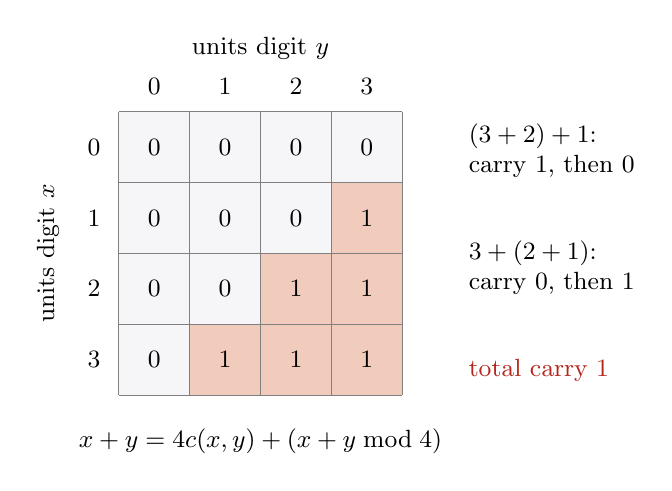
\begin{tikzpicture}[font=\small,>=stealth,x=0.9cm,y=0.9cm]
\foreach \x in {0,...,3} {
  \node at (\x+0.5,4.35) {$\x$};
  \node at (-0.35,3.5-\x) {$\x$};
  \foreach \y in {0,...,3} {
    \pgfmathtruncatemacro{\carry}{int((\x+\y)/4)}
    \ifnum\carry=1
      \fill[BrickRed!18] (\y,3-\x) rectangle (\y+1,4-\x);
    \else
      \fill[MidnightBlue!4] (\y,3-\x) rectangle (\y+1,4-\x);
    \fi
    \node at (\y+0.5,3.5-\x) {$\carry$};
  }
}
\draw[step=1,gray] (0,0) grid (4,4);
\node at (2,4.9) {units digit $y$};
\node[rotate=90] at (-1.0,2) {units digit $x$};
\node[align=left,anchor=west] at (4.8,3.45) {$(3+2)+1$:\\carry $1$, then $0$};
\node[align=left,anchor=west] at (4.8,1.8) {$3+(2+1)$:\\carry $0$, then $1$};
\node[anchor=west,BrickRed] at (4.8,0.35) {total carry $1$};
\node at (2,-0.65) {$x+y=4c(x,y)+(x+y\bmod4)$};
\end{tikzpicture}
